\section{Resultados}

O conjunto montado ficou como mostrado na figura \ref{montagem}:

\begin{figure}[h!]
\caption{Montagem do circuito}
\centering % para centralizarmos a figura
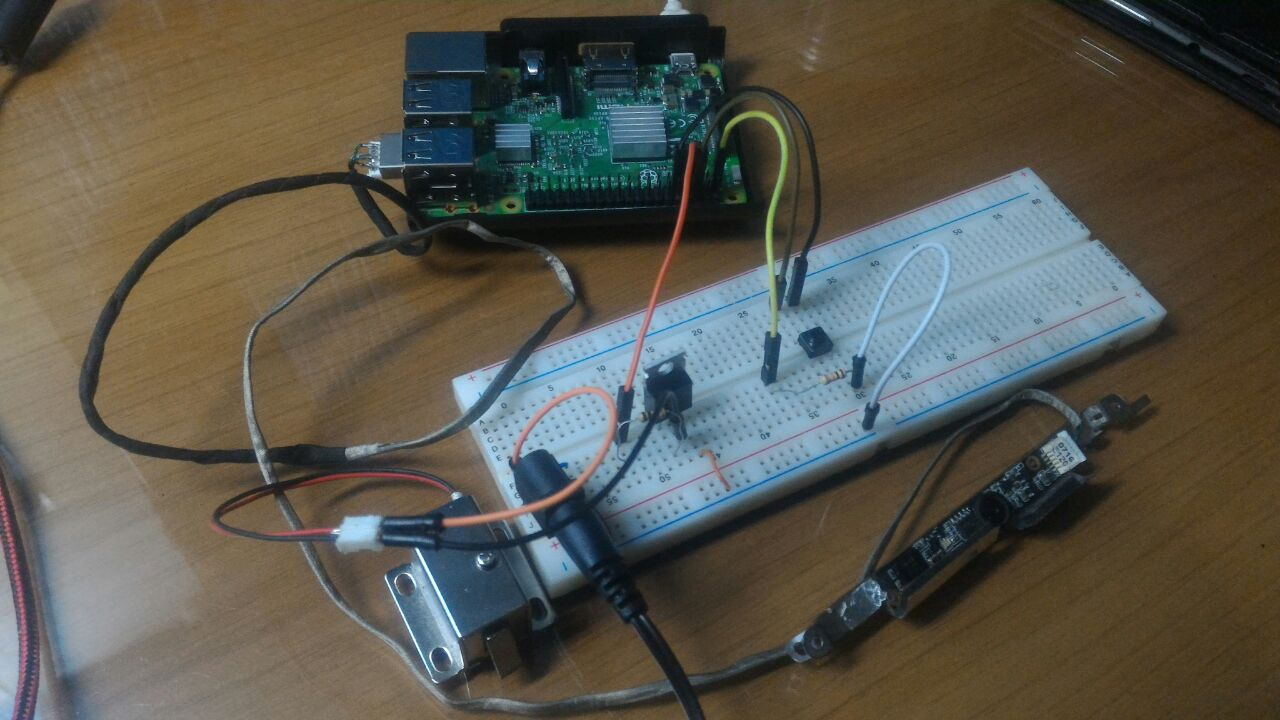
\includegraphics[width=8cm]{montagem.jpeg} % leia abaixo
\label{montagem}
\end{figure}


A ativa��o da trava eletr�nica foi realizada com sucesso, sem sobreaquecimento do transistor, nem falha na comunica��o.

Na parte de software realizamos os teste apenas no computador, pois algumas biblotecas n�o foram possiveis a usa instala��o na raspberry at� o momento. 

A figura \ref{bot} mostra o funcionamento da conversa do administrador do sistema com o Bot do Telegram.

\begin{figure}[h!]
\caption{BOT do Telegram e funcionamento.}
\centering % para centralizarmos a figura
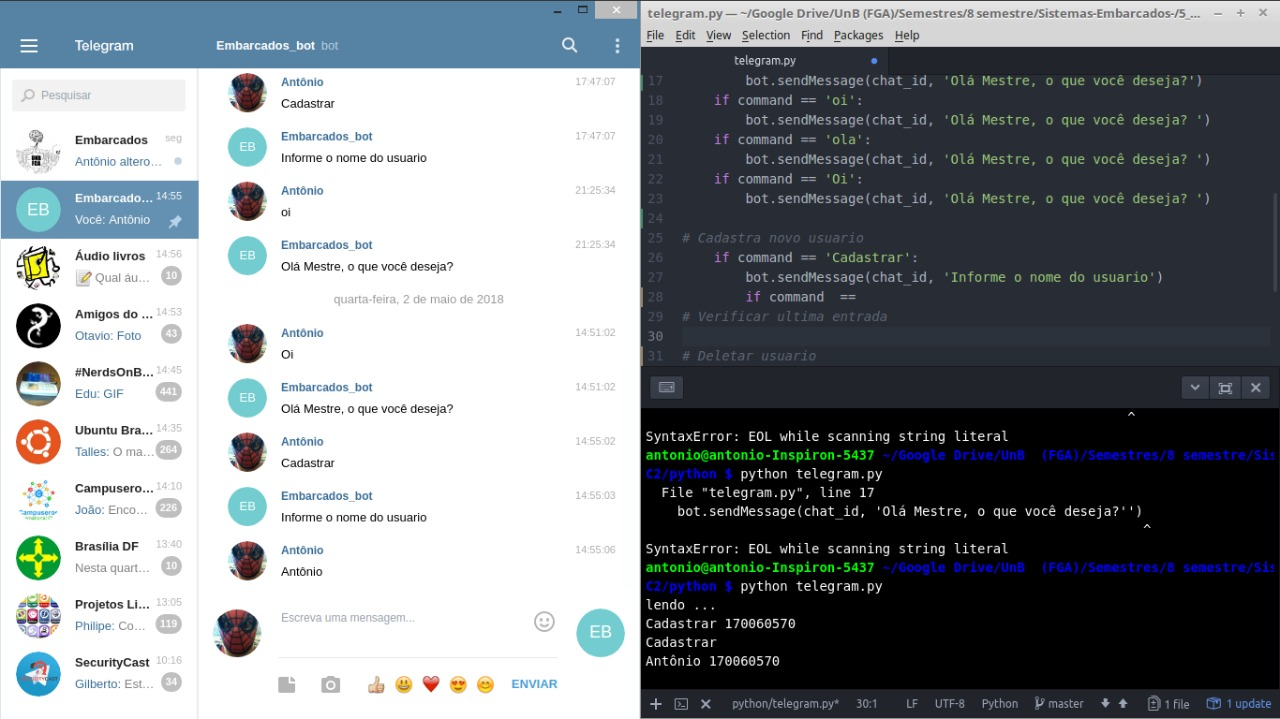
\includegraphics[width=8cm]{bot.jpeg} % leia abaixo
\label{bot}
\end{figure}

Na figura \ref{reconhecimento} pode ser visto o reconhecimento facial em funcionamento.

\begin{figure}[h!]
\caption{Reconhecimento facial em funcionamento funcionamento.}
\centering % para centralizarmos a figura
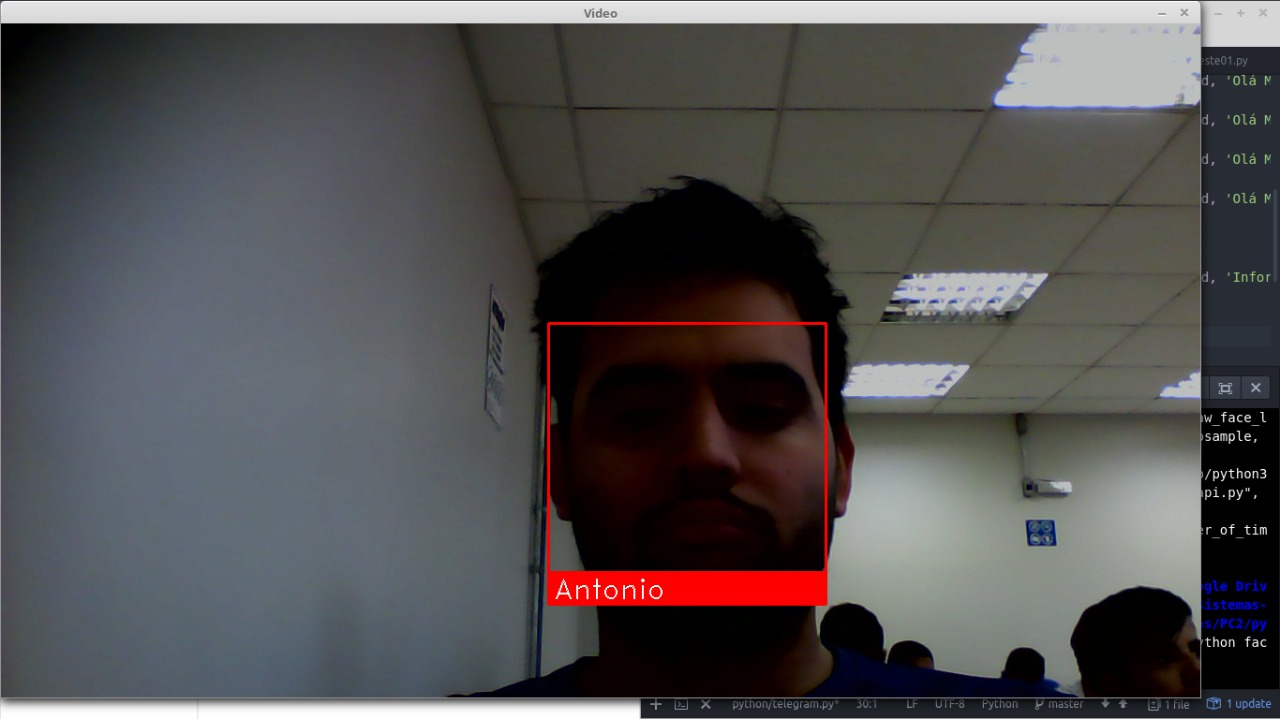
\includegraphics[width=8cm]{reconhecimento.jpeg} % leia abaixo
\label{reconhecimento}
\end{figure}



